

\section{Experimental Results and Discussion}
{\color{red}Lizhen, Gabriela and Nathan?}

As a reference, we compared our best results for each task with their corresponding benchmarks. 
For all the task, we reach a comparable performance to the state-of-the-art methods, except
for NER that we are 2.5 points below, because... (Table\ref{benchmark}).
However, in this paper, we do not aim to maximize the absolute performance of the tasks under 
study, but rather to study the impact of word embeddings for sequence tagging tasks under control settings.

\begin{table*}
\caption{Benchmark results vs. our best results}
\begin{center}
\begin{small}
\begin{tabular}{lll}
\hline
\textbf{Task} & \textbf{Benchmark} & \textbf{Us} \\ \hline
POS-Tagging & (Accuracy) 97.24 \cite{Toutanova:2003} & 0.9592 (skip-gram negsam+up) \\ 
Chunking & (F1) 0.9429 \cite{Sha:2003} & 0.9386 (Brown cluster v2000+)\\  
NER & (F1) 0.8931 \cite{Ando:2005} & 0.8686 (skip-gram negsam+noup)\\  
MWE & (F1) 0.6253 \cite{Schneider+:2014} & 0.6546 (cw+up)\\ 
\hline
\label{benchmark}
\end{tabular}
\end{small}
\end{center}
\end{table*}

Figure \ref{fig:bestPOS-Chunk} and Figure \ref{fig:bestNER-MWE} summarized the results 
obtained for each task and each word embedding method in heat-maps plots. 
Across the different tasks, we could not find any trend that tell which word embedding methods is the best and under which settings, since the difference between them are not significant (see that all methods are in green when all the available training data was used).

We observed also that word embeddings are especially helping POS-tagging and chunking when there are only 
several hundreds of training instances.
These early improvements are less evident for NER and MWE. 
We attribute this to: i) NER and MWE are more difficult tasks than POS-tagging and chunking;
ii) NER and MWE require more training data; iii) the performance of NER and MWE heavily dependent on complex features such as gazetteers and lexicons like Wordnet, which are not captured by the feature representation learned from unlabelled data, meanwhile the standard features used in POS-tagging and chunking (e.g., stemming) are more likely to be capture by the word embeddings, because...

% when the feature space is bigger the generalization power should be bigger
As expected, word embeddings and Brown clustering excel in out-of-domain performance.
% we dont have plots for that 

Fine-tuning can correct poorly learned word representations but can be
overfitted if unsupervisely learned ones are already good.

% something about OOV
% In Figure \ref{POS-OOV-IN} and Figure \ref{NER-OOV-OUT}

Because we can either update pre-trained word embeddings during training or not, through the evaluation, we want to answer the following questions:
\begin{itemize}
\item How well do different word embeddings perform in all tasks when supervised fine-tuning is \textit{not} performed?
\item How well do different word embeddings perform in all tasks when supervised fine-tuning is performed?
\item How does the size of labeled training data affect the experimental results?
\item How well do the word embeddings perform for unknown words? 
\item How do the key parameters of each word learning algorithms affect the experimental results?
\end{itemize}









%%%%%%%%%%%%%%%%%%%%%%%%%%%%
%%% HEATMAPS 
\clearpage

\begin{figure*}
\caption{Best results for each method for POS-Tagging and Chunking. The x-axis correspond to the different word embeddings methods and the y-axis to the 10 training partitions at log scale. Green color stand for high performance, while red color stands for low performance.}
\centering
\begin{subfigure}{7cm}
	\centering
    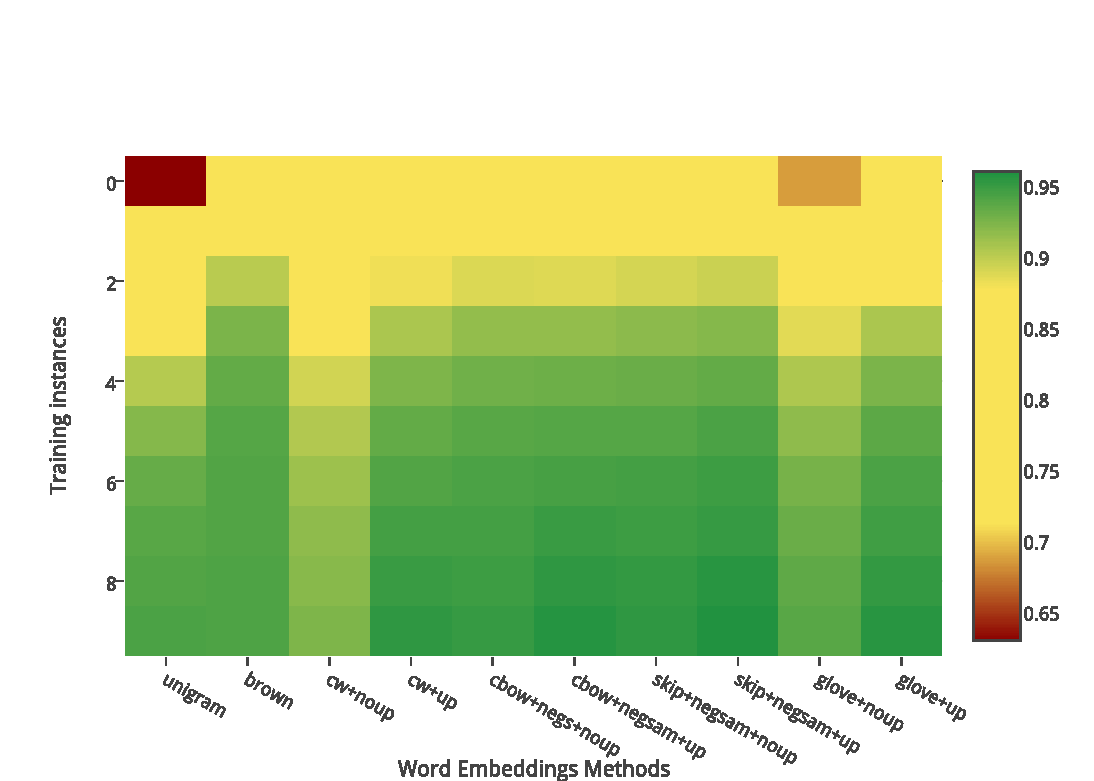
\includegraphics[scale=0.4]{plots/map-pos}    	
	\subcaption{POS-Tagging Accuracy}	
\end{subfigure}
\begin{subfigure}{7cm}
	\centering
    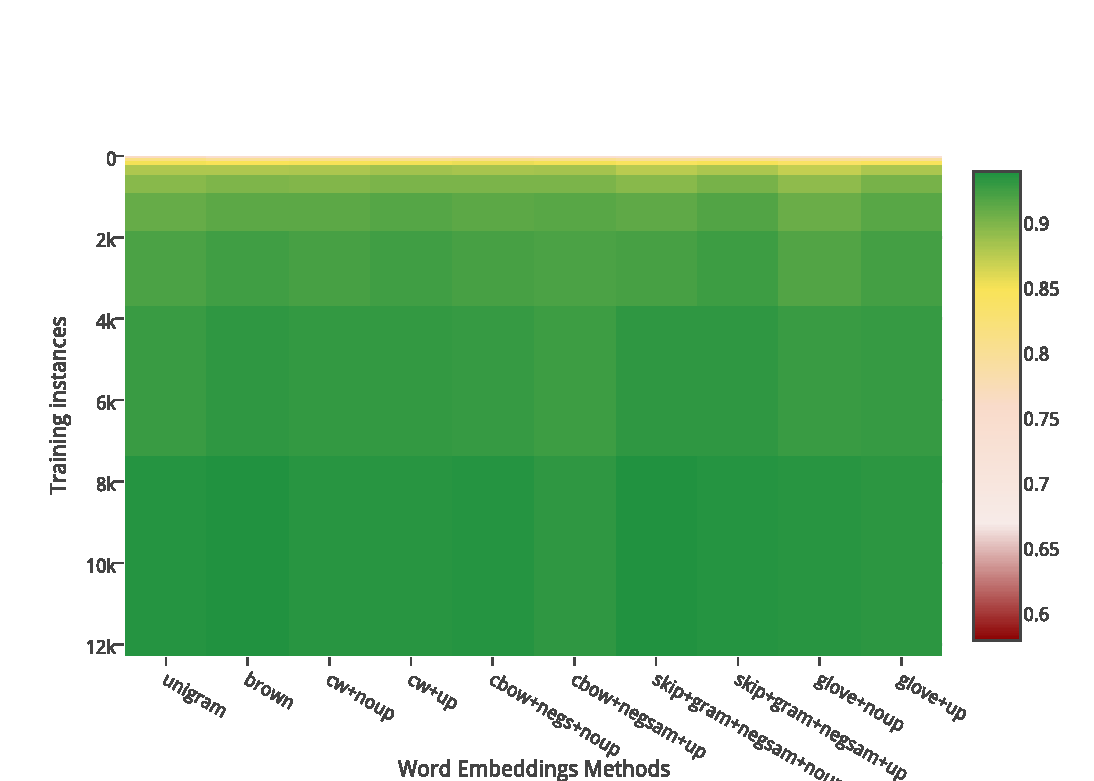
\includegraphics[scale=0.4]{plots/map-chunk}
	\subcaption{Chunking F1-Measure}	
\end{subfigure}
\label{fig:bestPOS-Chunk}
\end{figure*}

\begin{figure*}
\caption{Best results for each method for NER and MWE}
\centering
\begin{subfigure}{7cm}
	\centering
    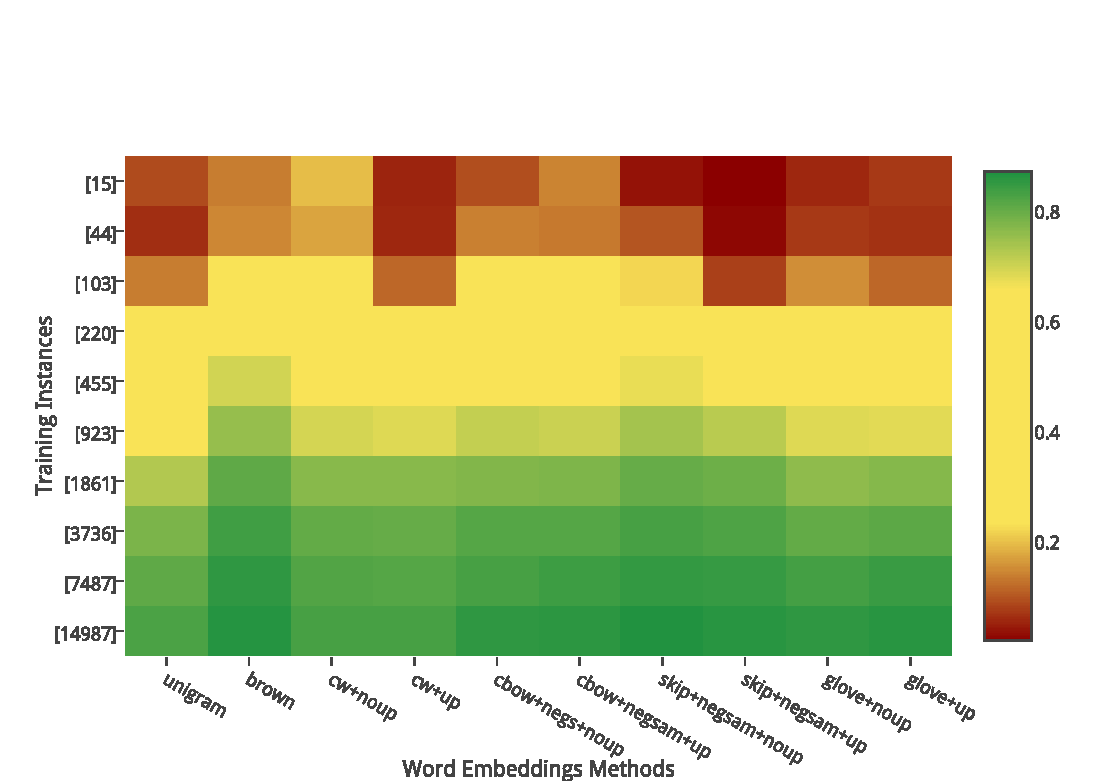
\includegraphics[scale=0.4]{plots/map-ner}    	
	\subcaption{NER F1-Measure}	
\end{subfigure}
\begin{subfigure}{7cm}
	\centering
    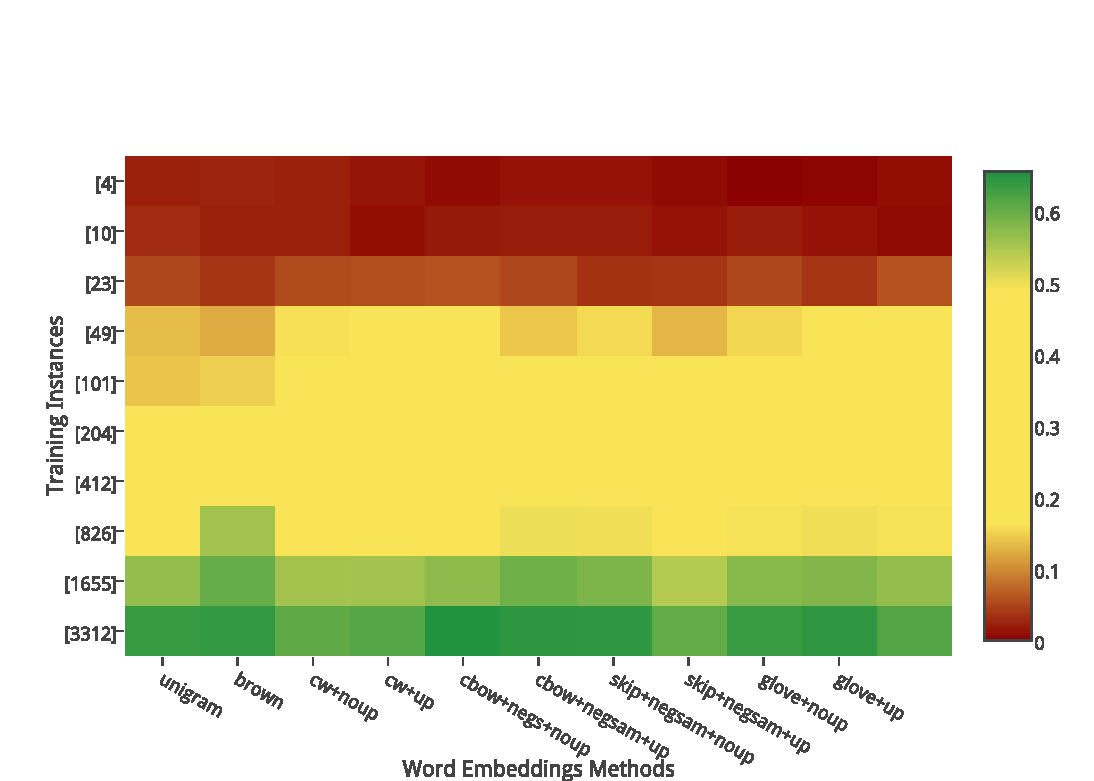
\includegraphics[scale=0.4]{plots/map-mwe}
	\subcaption{MWEs F1-Measure}		
\end{subfigure}
\label{fig:bestNER-MWE}
\end{figure*}

\clearpage

\iffalse
%%%%%%%%%%%%%%%%%%%%%%%%%%%%
%%% BEST in PLOTS
\begin{figure*}[h]
\caption{Best results for each method for POS-Tagging and Chunking}
\centering
\begin{subfigure}{6cm}
	\centering
    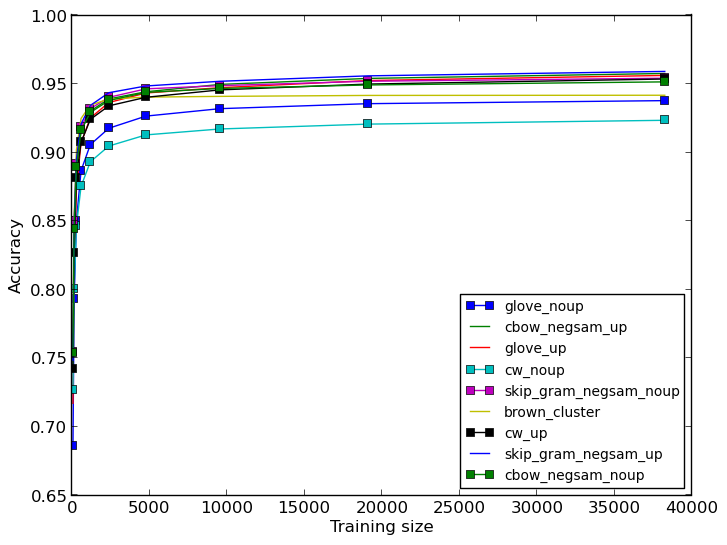
\includegraphics[scale=0.3]{plots/bestPOS}    	
	\label{fig:bestpos}
	\subcaption{POS-Tagging results}	
\end{subfigure}
\begin{subfigure}{6cm}
	\centering
    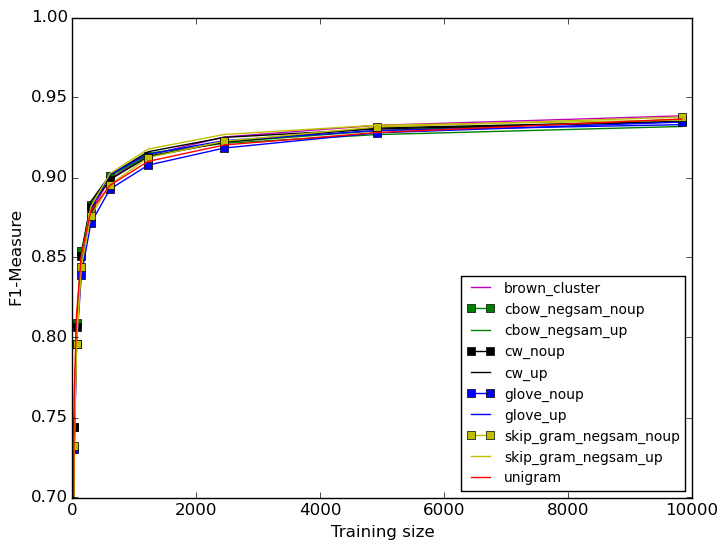
\includegraphics[scale=0.3]{plots/bestChunking}
	\label{fig:bestchunking}
	\subcaption{Chunking results}	
\end{subfigure}
\end{figure*}

\begin{figure*}[h]
\caption{Best results for each method for NER and MWE}
\centering
\begin{subfigure}{6cm}
	\centering
    	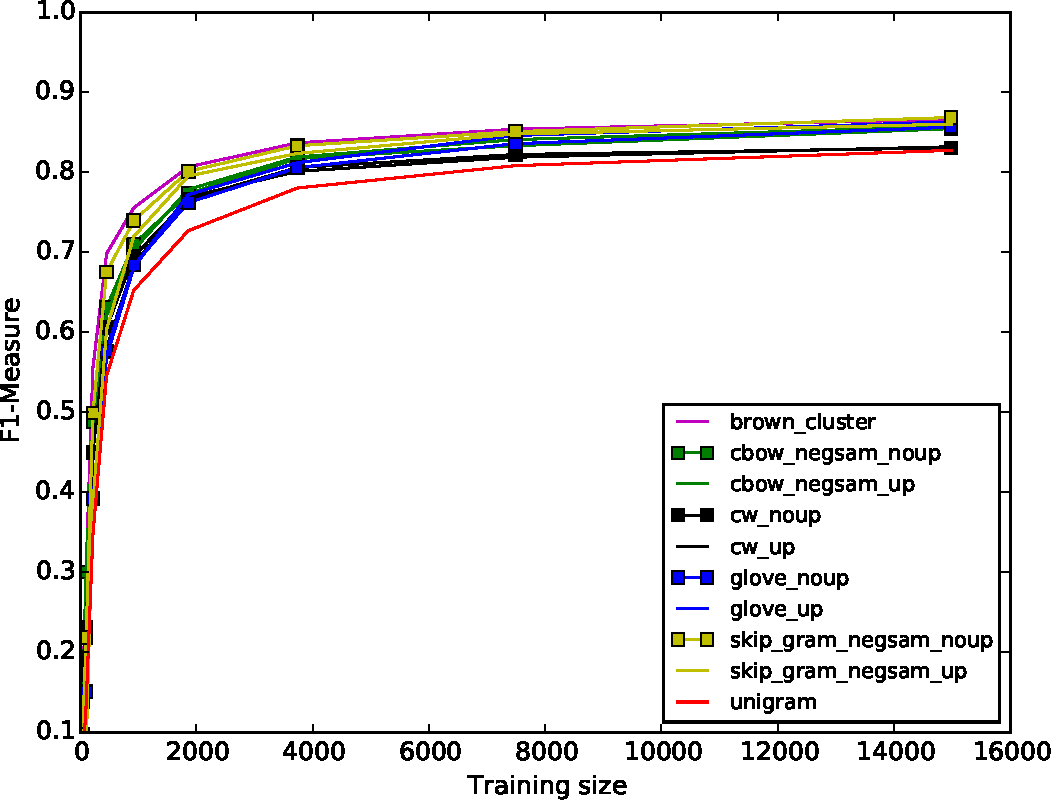
\includegraphics[scale=0.3]{plots/bestNER}
	\subcaption{NER results}	
	\label{fig:bestner}
\end{subfigure}
\begin{subfigure}{6cm}
	\centering
    	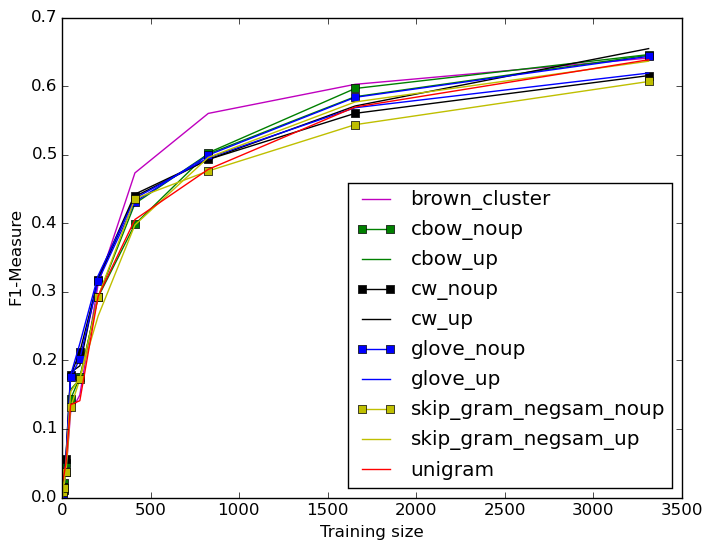
\includegraphics[scale=0.3]{plots/bestMWE}
    \subcaption{MWE results}	
	\label{fig:bestmwe}
\end{subfigure}  	
\end{figure*}  

\begin{figure*}[h]
\caption{Chunking and MWE out-of-vocabulary-words accuracy for \textit{in-domain} test set}
\centering
\begin{subfigure}{7cm}
	\centering
    	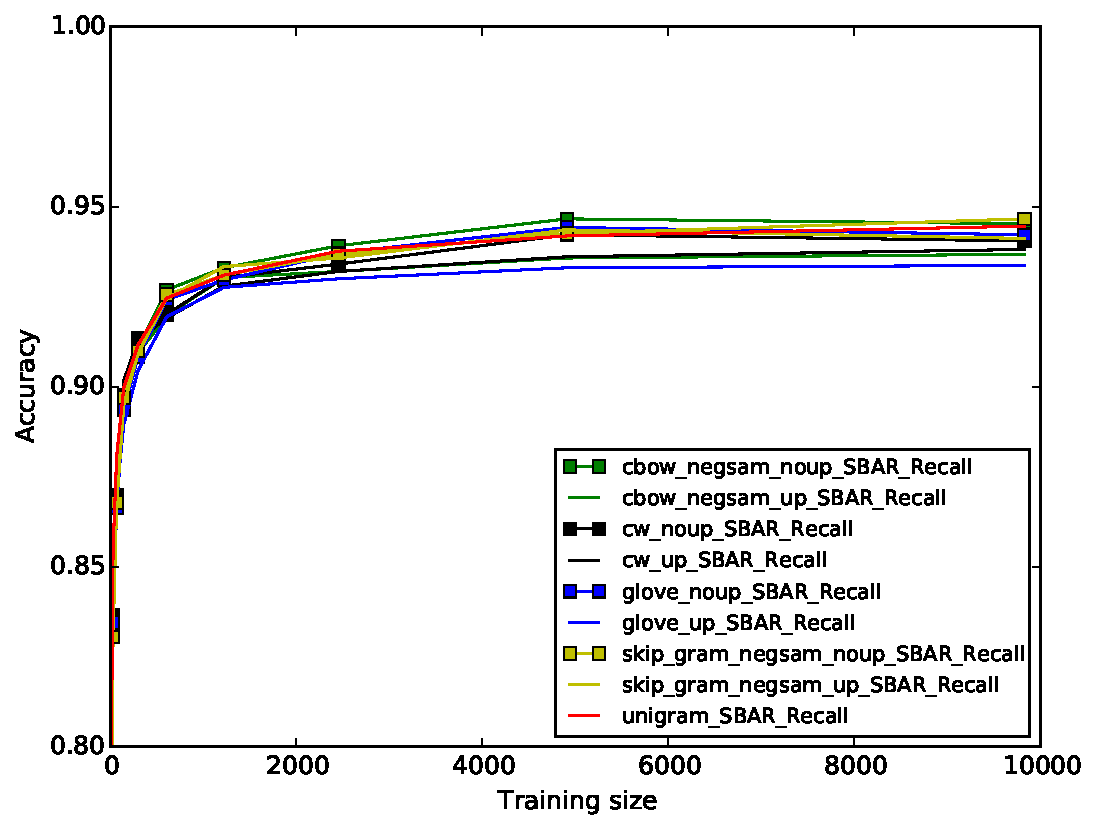
\includegraphics[scale=.4]{plots/Chunking-OOV}
    	\subcaption{Chunking accuracy for OOV}
	\label{fig:inner}
\end{subfigure}
\begin{subfigure}{7cm}
	\centering
    	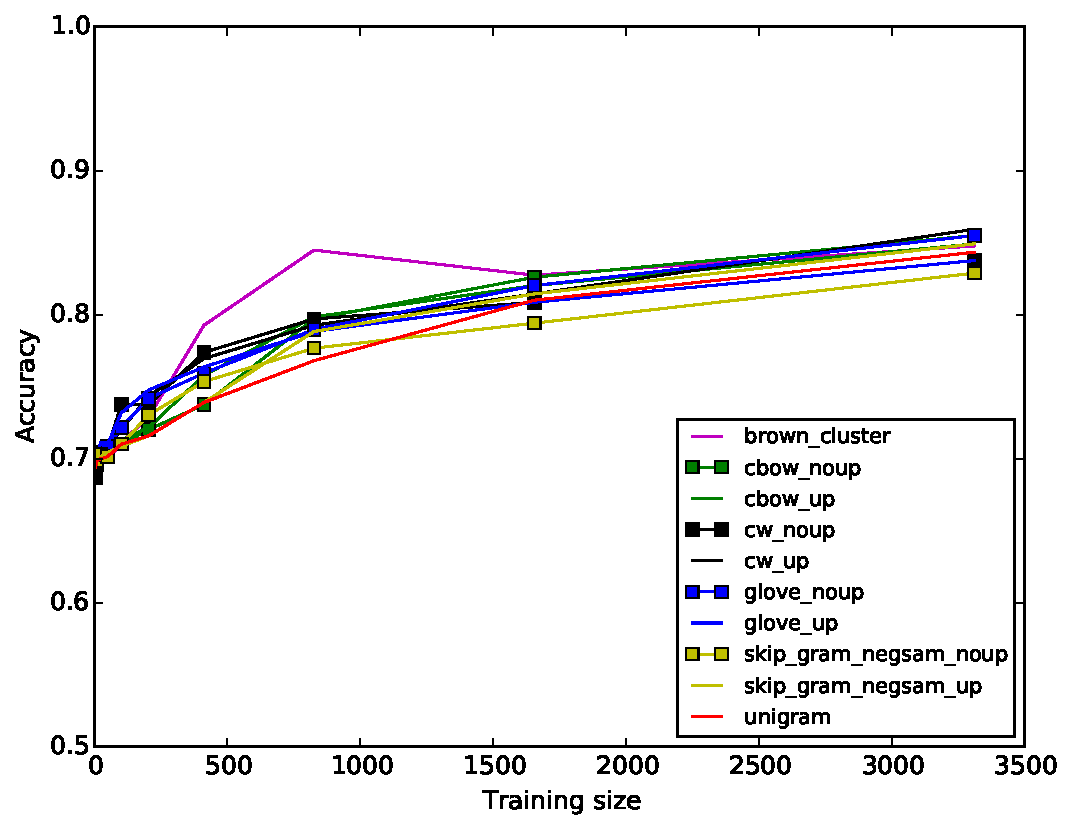
\includegraphics[scale=0.4]{plots/MWE-OOV}
   	\subcaption{MWE accuracy for OOV}
	\label{fig:outner}
\end{subfigure}  	
\end{figure*}	
\fi



%%%%%%%%%%%%%%%%%%%%%%%%%%%%
%%% OOV POS and NER
\begin{figure*}[ht] 
%\caption{Out-of-vocabulary-words (OOV) accuracy for \textit{in-domain} and \textit{out-of-domain} test sets}
\label{OOV} 
  \begin{minipage}[b]{7cm}
    	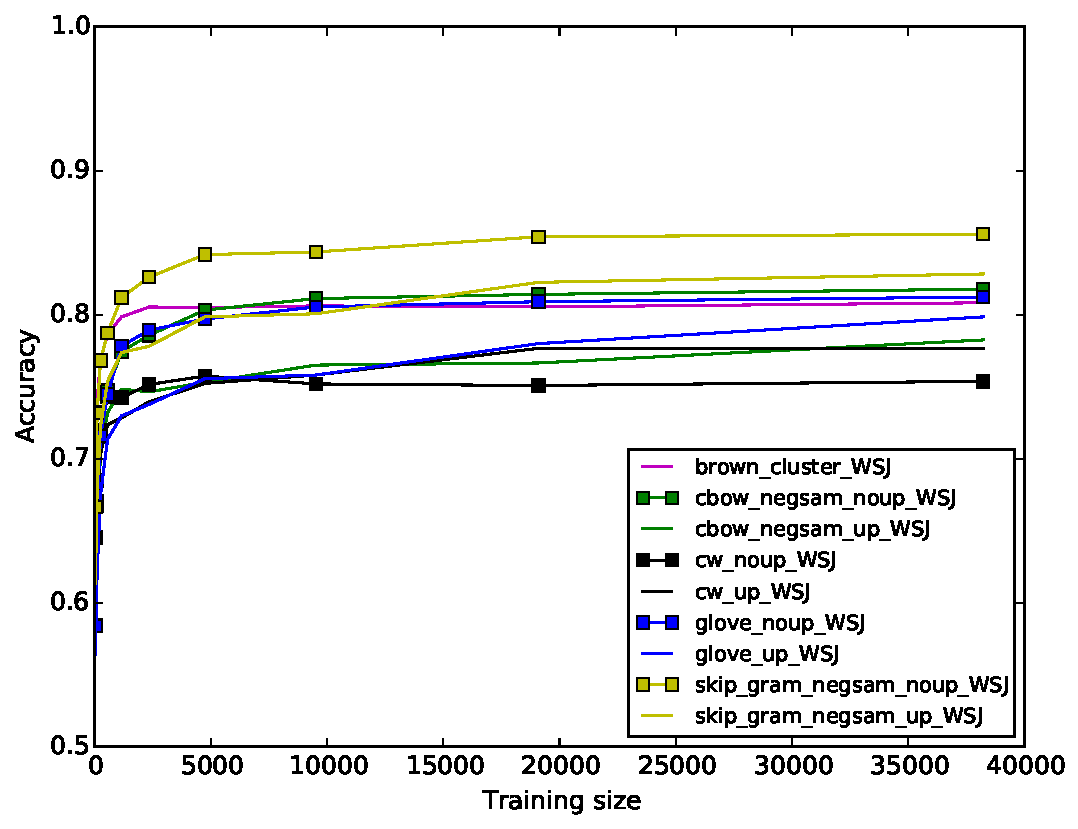
\includegraphics[scale=0.4]{plots/POS-OOV-IN}
    \caption{POS-Tagging accuracy for \textit{in domain} OOV} 
    \label{POS-OOV-IN}	
  \end{minipage} 
  \begin{minipage}[b]{7cm}
    	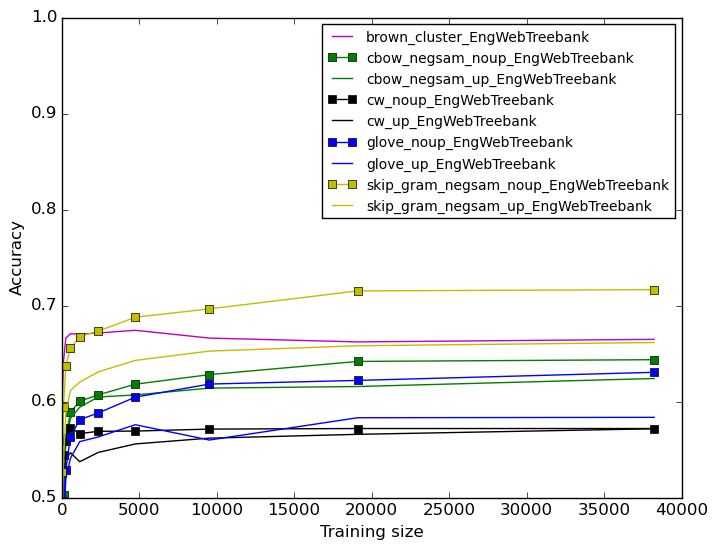
\includegraphics[scale=0.4]{plots/POS-OOV-OUT}
    \caption{POS-Tagging accuracy for \textit{out domain} OOV} 
    \label{POS-OOV-OUT}	
  \end{minipage} 
  \begin{minipage}[b]{7cm}
    	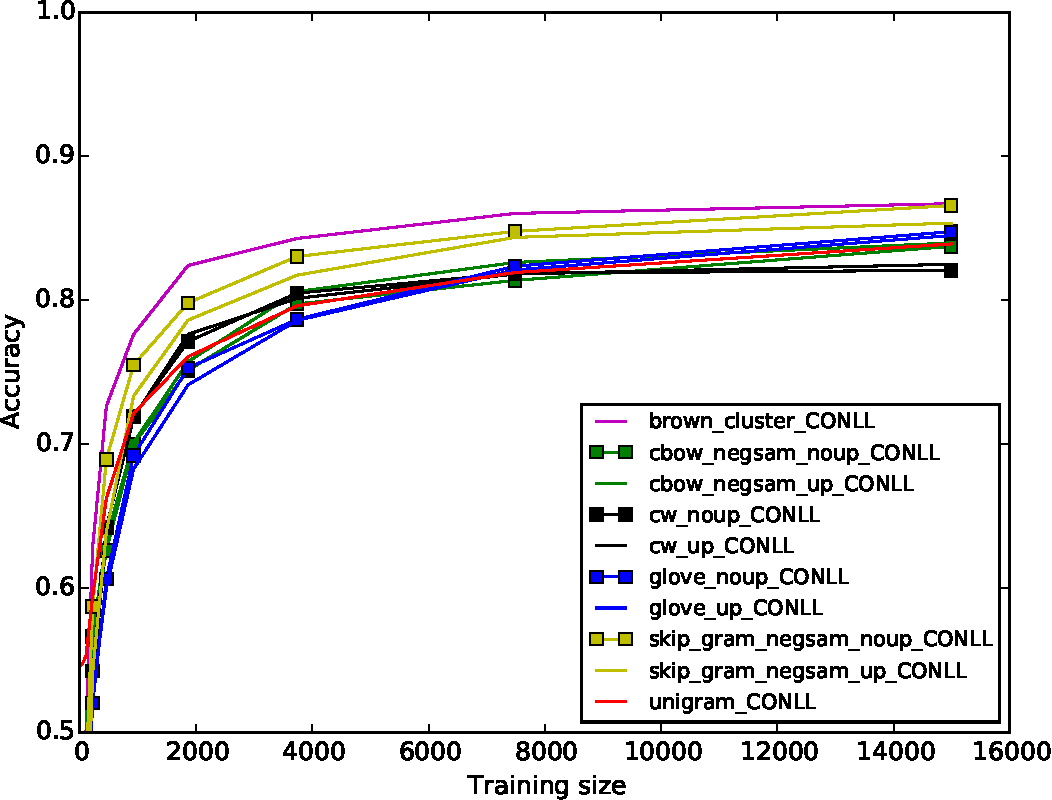
\includegraphics[scale=0.4]{plots/NER-OOV-IN}
    \caption{NER accuracy for \textit{out domain} OOV} 
    \label{NER-OOV-IN}
  \end{minipage}
  \hfill
  \begin{minipage}[b]{7cm}
    	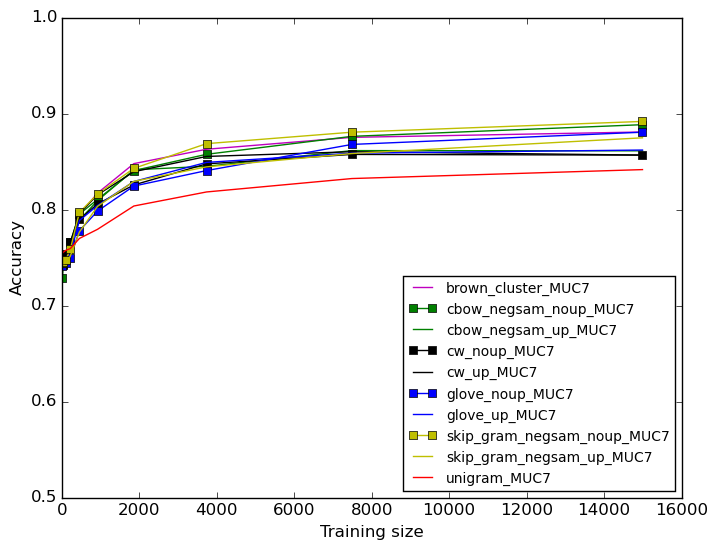
\includegraphics[scale=0.4]{plots/NER-OOV-OUT}
    \caption{NER accuracy for \textit{out domain} OOV} 
    \label{NER-OOV-OUT}
  \end{minipage} 
  \begin{minipage}[b]{7cm}
    	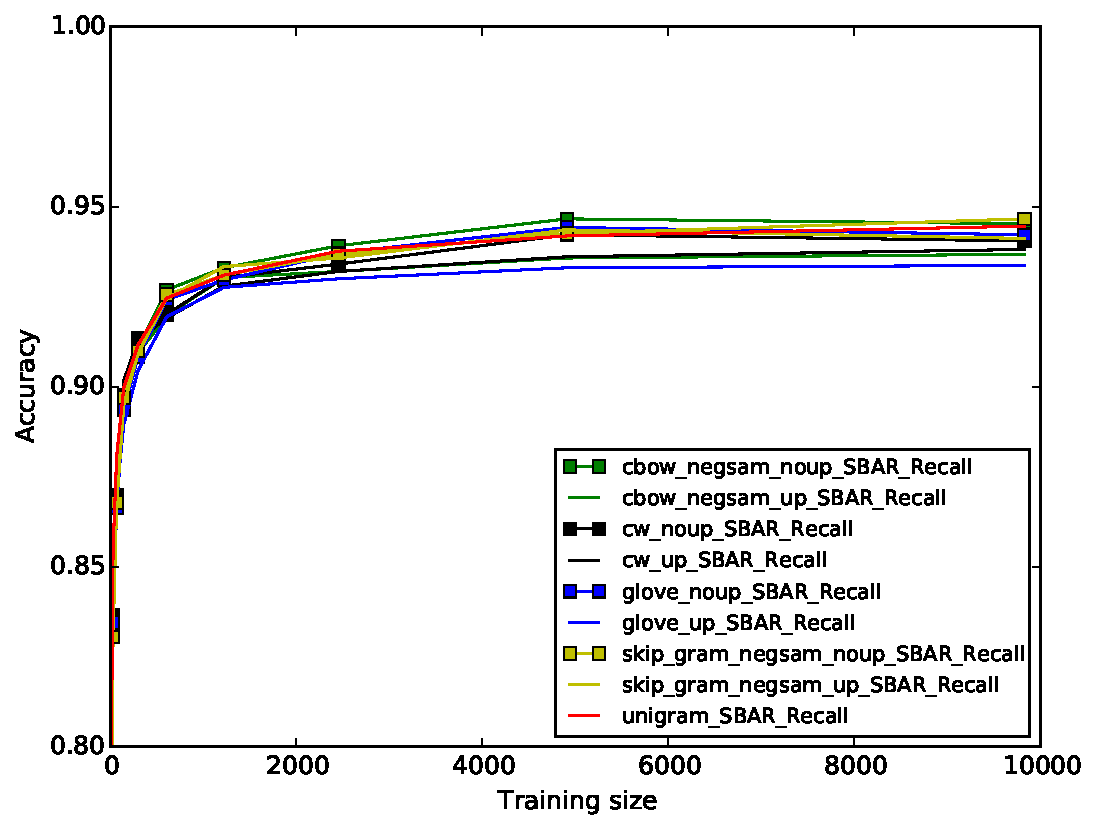
\includegraphics[scale=0.4]{plots/Chunking-OOV}
    \caption{Chunking accuracy for OOV \textit{in domain} OOV} 
    \label{chunk-OOV}
  \end{minipage} 
    \hfill
  \begin{minipage}[b]{7cm}
    	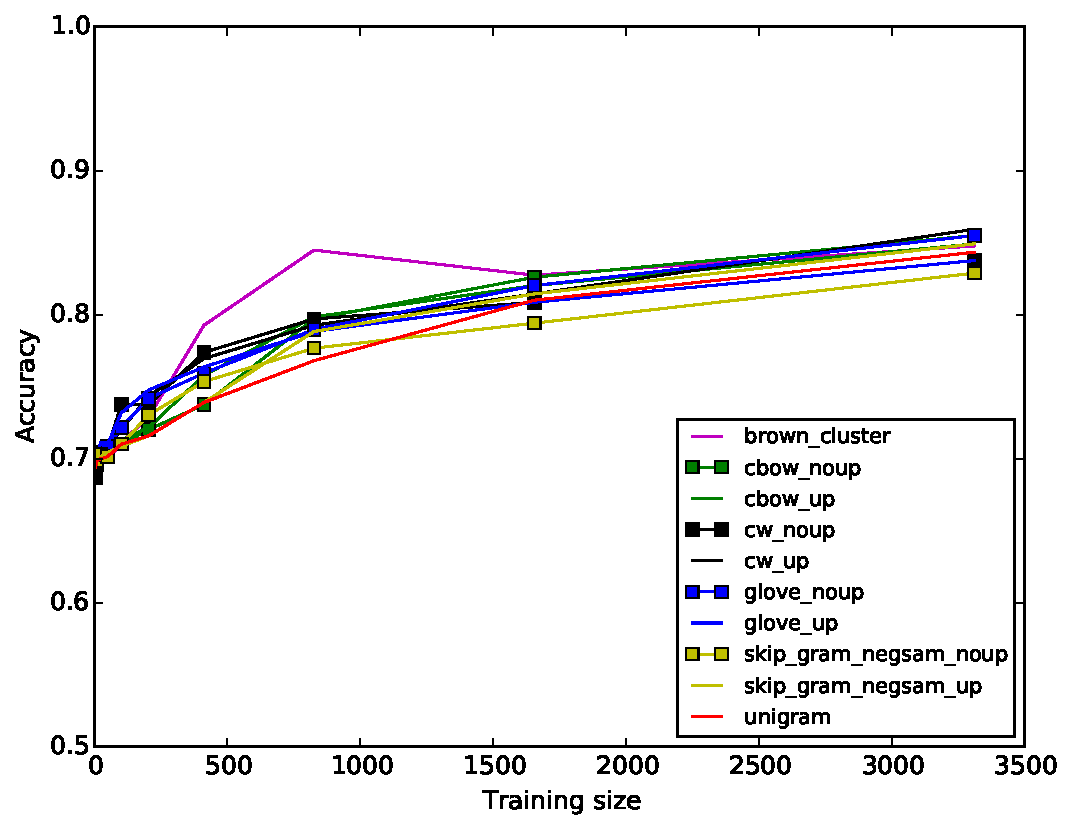
\includegraphics[scale=0.4]{plots/MWE-OOV}
     \label{POS-OOV}
    \caption{MWE accuracy for \textit{out domain} OOV} 
  \end{minipage}   
\end{figure*}









\subsection{Result tables}

The first column of each table contains the number of training sentences.

\subsubsection{Best hyperparameters for All Tasks}

\begin{table*}[h]
\centering
\begin{adjustbox}{max width=\textwidth}
\pgfplotstabletypeset[col sep=comma, 
precision=4,
every head row/.style={
before row=\toprule,
after row=\midrule},
every last row/.style={
after row=\bottomrule
}]{eval_results/key_results/POS/Accuracy.csv}
\end{adjustbox}
\caption{Accuracy of POS tagging evaluated on WSJ test set}
\label{table:accuracy_pos}
\end{table*}

\begin{table*}[h]
\centering
\begin{adjustbox}{max width=\textwidth}
\pgfplotstabletypeset[col sep=comma, 
precision=4,
every head row/.style={
before row=\toprule,
after row=\midrule},
every last row/.style={
after row=\bottomrule
}]{eval_results/key_results/NER/CONLL_F1Measure.csv}
\end{adjustbox}
\caption{F1 Measure of NER evaluated on CoNLL test set}
\label{table:f1_ner}
\end{table*}

\begin{table*}[h]
\centering
\begin{adjustbox}{max width=\textwidth}
\pgfplotstabletypeset[col sep=comma, 
precision=4,
every head row/.style={
before row=\toprule,
after row=\midrule},
every last row/.style={
after row=\bottomrule
}]{eval_results/key_results/chunking/chunks_F1Measure.csv}
\end{adjustbox}
\caption{F1 Measure of chunking evaluated on CoNLL test set}
\label{table:f1_chunking}
\end{table*}

\begin{table*}[h]
\centering
\begin{adjustbox}{max width=\textwidth}
\pgfplotstabletypeset[col sep=comma, 
precision=4,
every head row/.style={
before row=\toprule,
after row=\midrule},
every last row/.style={
after row=\bottomrule
}]{eval_results/key_results/MWEs/mwe_F1Measure.csv}
\end{adjustbox}
\caption{F1 Measure of MWE identification evaluated on MWE test set}
\label{table:f1_mwe}
\end{table*}

\subsubsection{Out of Vocabulary results for All Tasks}

\begin{table*}[h]
\centering
\begin{adjustbox}{max width=\textwidth}
\pgfplotstabletypeset[col sep=comma, 
precision=4,
every head row/.style={
before row=\toprule,
after row=\midrule},
every last row/.style={
after row=\bottomrule
}]{eval_results/key_results/POS/WSJ_out-of-vocabulary_Accuracy.csv}
\end{adjustbox}
\caption{Accuracy of POS tagging evaluated on out-of-vocabulary words in WSJ test set}
\label{table:outVocab_pos_accuracy}
\end{table*}

\begin{table*}[h]
\centering
\begin{adjustbox}{max width=\textwidth}
\pgfplotstabletypeset[col sep=comma, 
precision=4,
every head row/.style={
before row=\toprule,
after row=\midrule},
every last row/.style={
after row=\bottomrule
}]{eval_results/key_results/NER/CONLL_out-of-vocabulary_Accuracy.csv}
\end{adjustbox}
\caption{Accuracy of NER evaluated on out-of-vocabulary words in CoNLL test set}
\label{table:outVocab_ner_accuracy}
\end{table*}

\begin{table*}[h]
\centering
\begin{adjustbox}{max width=\textwidth}
\pgfplotstabletypeset[col sep=comma, 
precision=4,
every head row/.style={
before row=\toprule,
after row=\midrule},
every last row/.style={
after row=\bottomrule
}]{eval_results/key_results/chunking/Accuracy.csv}
\end{adjustbox}
\caption{Accuracy of Chunking evaluated on out-of-vocabulary words in CoNLL test set}
\label{table:outVocab_chunking_accuracy}
\end{table*}

\begin{table*}[h]
\centering
\begin{adjustbox}{max width=\textwidth}
\pgfplotstabletypeset[col sep=comma, 
precision=4,
every head row/.style={
before row=\toprule,
after row=\midrule},
every last row/.style={
after row=\bottomrule
}]{eval_results/key_results/MWEs/out-of-vocabulary_Accuracy.csv}
\end{adjustbox}
\caption{Accuracy of MWE identification evaluated on out-of-vocabulary words in MWE test set}
\label{table:outVocab_mwe_accuracy}
\end{table*}

\subsubsection{Out of domain Results for NER and POS}

\begin{table*}[h]
\centering
\begin{adjustbox}{max width=\textwidth}
\pgfplotstabletypeset[col sep=comma, 
precision=4,
every head row/.style={
before row=\toprule,
after row=\midrule},
every last row/.style={
after row=\bottomrule
}]{eval_results/key_results/POS/EngWebTreebank_Accuracy.csv}
\end{adjustbox}
\caption{Accuracy of POS tagging evaluated on English web treebank.}
\label{table:outDomain_accuracy_pos}
\end{table*}

\begin{table*}[h]
\centering
\begin{adjustbox}{max width=\textwidth}
\pgfplotstabletypeset[
col sep=comma, 
precision=4,
every head row/.style={
before row=\toprule,
after row=\midrule},
every last row/.style={
after row=\bottomrule
}]{eval_results/key_results/NER/MUC7_chunks_F1Measure.csv}
\end{adjustbox}
\caption{F1 measure of NER evaluated on MUC7 test set}
\label{table:outDomain_ner_f1}
\end{table*}


\section{Conclusion}
